% LAST UPDATED FOR MCP2017

\documentclass{beamer}
\usecolortheme[RGB={112,41,99}]{structure}
\usetheme{Berkeley}
\setbeamercovered{invisible}

\setbeamertemplate{frametitle continuation}{}

\usepackage{graphicx}
\usepackage{booktabs}
\usepackage{natbib}
\usepackage{lmodern}
\usepackage{tikz}
\usetikzlibrary{calc}
\usepackage{xcolor}
\definecolor{mid_purple}{HTML}{B894B1}

\title[Verifying Winner]{Rank Verification in Exponential Families}

\author[Kenneth Hung]{Kenneth Hung}
\institute[UC Berkeley]{
University of California, Berkeley \\
\medskip
\textit{kenhung@berkeley.edu}
}
\date{June 23, 2017 @ MCP2017}

\begin{document}

\begin{frame}
\titlepage
\end{frame}

\section{Introduction \& Motivation}

\begin{frame}{Introduction}
\begin{itemize}
\item Joint work with my advisor, Will Fithian
\item Paper available on arXiv:1610.03944
\end{itemize}
\end{frame}

\begin{frame}{A polling problem}
\begin{table}[htbp]
\centering
\begin{tabular}{c c c c}
	\hline
	Rank & Candidate & Result & Votes \\
	\hline
	$1$ & Trump & $31\%$ & $276$ \\
	$2$ & Cruz & $24\%$ & $214$ \\
	$3$ & Rubio & $17\%$ & $151$ \\
	$4$ & Carson & $8\%$ & $71$ \\
	$5$ & Paul & $4\%$ & $36$ \\
	$6$ & Bush & $4\%$ & $36$ \\
	$7$ & Huckabee & $3\%$ & $27$ \\
	$\vdots$ & $\vdots$ & $\vdots $ & $\vdots$ \\
	\hline
\end{tabular}
\caption{Simplified results from a February 1, 2016 Quinnipiac University poll of $890$ Iowa Republicans.}
\label{tbl:poll}
\end{table}
\end{frame}

\begin{frame}{A polling problem}
Questions that one might ask, {\it post hoc}:
\begin{itemize}
\item Verifying winner as best: Does Trump have the largest support?
\begin{itemize}
\item a.k.a.\ multiple comparison with sample best (CSB) in \citet{Stefansson:1988wj}
\end{itemize}
\item By how much: How much larger is Trump's support compared to other candidates?
\item Verifying other ranks: Does Cruz (Rubio, etc.) have the second (third, etc.) largest support? 
\end{itemize}
\end{frame}

\begin{frame}{A polling problem}
Two fundamental problems here:
\begin{enumerate}
	\item Only asking ``Is Trump the best?'' when Trump is winning --- selective inference
	\item Testing all pairwise hypotheses that Trump is better than Cruz, Rubio, Carson, etc. --- multiple comparison
\end{enumerate}
\end{frame}

\begin{frame}{Related work}
\begin{itemize}
\item Ranking and selection: \citet{Gupta:1971wk,Gupta:1985bj,Gutmann:1987fk}
\item Location-scale families: \citet{Gutmann:1987fk,Bofinger:1991hv,Maymin:1992fz,Karnnan:2009iv}
\item CSB for location family using partition: \citet{Stefansson:1988wj}
\item Multinomial families: \citet{Gupta:1967wg,Gupta:1976vd,Berger:1980ev,Nettleton:2009ht,Gupta:1989fe,Ng:2007cn,Gupta:1967wg}

\item Conditional selective inference: \citet{Fithian:2014ws}
\end{itemize}
\end{frame}

\section{Procedure}

\begin{frame}{A na\"ive approach}
\begin{itemize}
\item Verifying winner as best: One-tailed level-$\alpha$ test comparing Trump to Cruz
\item By how much: Invert the test above
\item Verifying other ranks: One-tailed level-$\alpha$ test comparing first runner-up to second runner-up, etc., using a step-down procedure.
\end{itemize}
\end{frame}

\begin{frame}{A valid, yet simple, approach}
\begin{itemize}
\item Verifying winner as best: {\bf Two}-tailed level-$\alpha$ test comparing Trump to Cruz
\item By how much: Invert the test above
\item Verifying other ranks: {\bf Two}-tailed level-$\alpha$ test comparing first runner-up to second runner-up, etc., using a step-down procedure
\end{itemize}
\end{frame}

\section{Technicalities}

\begin{frame}{Exponential families}
\begin{align*}
&~ p(x_1, \ldots, x_n; \theta_1, \ldots, \theta_n) \\
= &~ \exp(\theta_1 x_1 + \cdots + \theta_n x_n - \log A(\theta_1, \ldots, \theta_n)) h(x_1, \ldots, x_n)
\end{align*}
\begin{itemize}
\item $x_i$ are the observations
\item $\theta_i$ are the natural parameter being ranked and tested
\item $h(\cdot)$ is the carrier distribution
\item $A(\cdot)$ is the normalizing constant
\end{itemize}
\end{frame}

\begin{frame}{Schur-concave exponential families}
\begin{itemize}
\item Schur-concave exponential families require $h$ to be Schur-concave
\item Generalization and relaxation of log-concave exponential family to potentially multivariate, discrete distributions
\item If $x \succeq y$ is the majorization order, then
\[
h(x) \le h(y).
\]
\end{itemize}
\end{frame}

\begin{frame}{Examples}
\begin{itemize}
\item Independent binomial treatment outcomes in a clinical trial
\item Competitive sports under the Bradley--Terry model
\item Comparing the variances of independent normal populations
\end{itemize}
\end{frame}

\section{Proof Sketches}

\begin{frame}{Key ideas in proof}
\begin{enumerate}
\item Selective inference: Conditioning on the selection event \citep{Fithian:2014ws}
\item Multiple comparison: Union null, only largest $p$-value needed
\end{enumerate}
\end{frame}

\begin{frame}{Selective inference}
\begin{itemize}
\item Question only asked about candidate $i$ when $X_i > X_j$ for all $j \ne i$
\item The corresponding event is thus
\[
\{X_i > \max_{i \ne j} X_j\}
\]
\end{itemize}
\end{frame}

\begin{frame}{Multiple comparison}
\begin{itemize}
\item Construct a $p$-value $p_{ij}$ for the winner against each candidate
\item The null ``the winner is not the best'' is a union null
\item Suffices to look at the largest $p$-values
\item Suffices to show that the largest $p$-value is obtained by comparing the winner and the runner-up
\end{itemize}
\end{frame}

\begin{frame}{Nuisance parameters}
In constructing $p_{ij}$,
\begin{itemize}
\item Parameter of interest: $\theta_i - \theta_j$
\item Nuisance parameters: $\theta_i + \theta_j$, and $\theta_k$ for all $k \ne i, j$
\item Condition on $2M_{ij} = X_i + X_j$, $X_{\setminus\{i, j\}}$.
\item Use $2D_{ij} = X_i - X_j$ as the test statistic
\end{itemize}
\end{frame}

\begin{frame}{Proof by pictures}
\begin{itemize}
\item Graphical representation of $p_{ij}$ and $p_{ik}$ for comparison
\item WLOG assume that $i = 1$ is the winner, $j = 2$ is the runner-up, and $k = 3$
\item Under the conditioning, $X_1 + X_2 + X_3$ and $X_{\setminus\{1, 2, 3\}}$ are held constant
\item Everything can fit on a 2D picture!
\end{itemize}
\end{frame}

\begin{frame}{Proof by pictures}
\centering
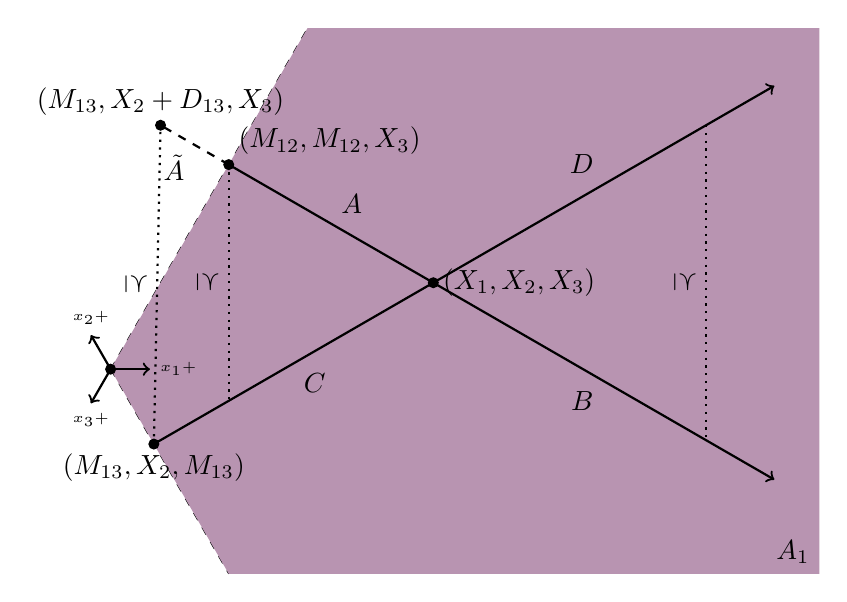
\begin{tikzpicture}
	\coordinate (C1) at (60:5);
	\coordinate (C2) at (300:3);
	\coordinate (A) at (60:3);
	\coordinate (B) at ($(A) + (330:3)$);
	\coordinate (C) at ($(0, 0)!(B)!(C2)$);
	\coordinate (D) at ($(A) + (150:1)$);
	\draw[dashed] (0, 0) -- (C1);
	\draw[dashed] (0, 0) -- (C2);
	\fill[mid_purple] (0, 0) -- (C1) -- ($(C1) + (6.5, 0)$) -- ($(C2) + (7.5, 0)$) -- (C2) -- cycle;
	\node[above left] at ($(C2) + (7.5, 0)$) {$A_1$};
	\draw[thick] (A) -- (B) node[midway, above right] {$A$};
	\draw[thick, ->] (B) -- ++(330:5) node[midway, below left] {$B$};
	\fill (A) circle(2pt) node[above right] {$\left(M_{12}, M_{12}, X_3\right)$};
	\fill (B) circle(2pt) node[right] {$\left(X_1, X_2, X_3\right)$};
	\fill (0, 0) circle(2pt);
	\draw[thick, ->] (0, 0) -- (0.5, 0) node[right] {\tiny $x_1 +$};
	\draw[thick, ->] (0, 0) -- (120:0.5) node[above] {\tiny $x_2 +$};
	\draw[thick, ->] (0, 0) -- (240:0.5) node[below] {\tiny $x_3 +$}; \pause
	\draw[thick] (C) -- (B) node[midway, below right] {$C$};
	\node[below] at (C) {$\left(M_{13}, X_2, M_{13}\right)$};
	\draw[thick, ->] (B) -- ++(30:5) node[midway, above left] {$D$};
	\fill ($(0, 0)!(B)!(C2)$) circle(2pt); \pause
	\draw[thick, dashed] (A) -- (D) node[midway, below left] {$\tilde{A}$};
	\fill (D) circle(2pt) node[above] {$\left(M_{13}, X_2 + D_{13}, X_3\right)$};
	\draw[thick, dotted] (C) -- (D) node[midway, below, rotate=-90] {$\succeq$};
	\draw[thick, dotted] (A) -- ++(0, -3) node[midway, below, rotate=-90] {$\succeq$};
	\draw[thick, dotted] ($(B) + (30:4)$) -- ($(B) + (330:4)$) node[midway, below, rotate=-90] {$\succeq$};
\end{tikzpicture}
\end{frame}

\begin{frame}{Power comparison}
\begin{itemize}
\item \citet{Gupta:1967wg} provided a subset selection procedure for the multinomial problem
\item Can be used as a test for if the winner is the best
\item Tested on parameters in form of
\[
(e^\delta, \underbrace{1, 1, \ldots, 1}_{n - 1})
\]
\end{itemize}
\end{frame}

\begin{frame}{Power comparison}
\centering
\includegraphics[width=0.95\textwidth]{multinomial-power.png}
\end{frame}

\begin{frame}[allowframebreaks]{References}
\footnotesize{\bibliography{papers}\bibliographystyle{plainnat}}
\end{frame}

\begin{frame}
\centering
{\Large Thanks!}
\end{frame}

\end{document}